\renewcommand{\theequation}{\theenumi}
\begin{enumerate}[label=\thesection.\arabic*.,ref=\thesection.\theenumi]
\numberwithin{equation}{enumi}

\item Draw Fig. \ref{fig:quadeq}.

\begin{figure}[!ht]
\centering
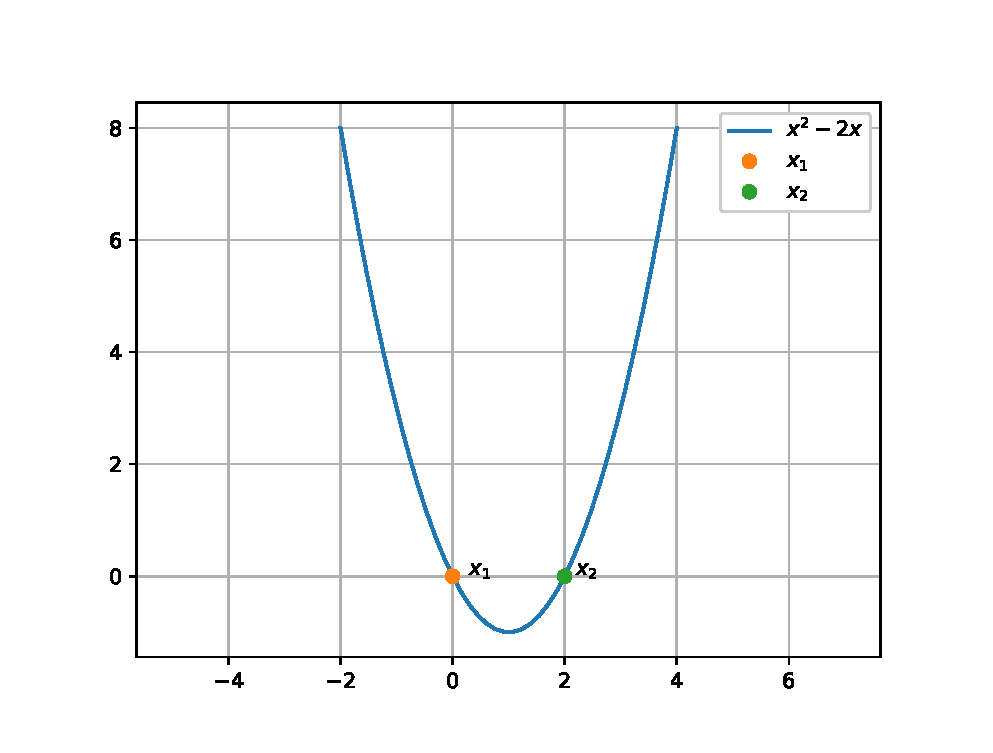
\includegraphics[width=\columnwidth]{./figs/quadratic_equation.eps}
\caption{$x^2 -2x$ generated using python}
\label{fig:quadeq}
\end{figure} 

\solution The  following Python code generates Fig. \ref{fig:quadeq}

\begin{lstlisting}
codes/conics.py
\end{lstlisting}
\end{enumerate}

